Um mögliche vorhandene Ungleichgewichte auszugleichen, haben die Probanden in diesem Projekt drei Ausgleichsübungen trainiert.
Diese dienen dem Muskelaufbau und sollen die Beweglichkeit verbessern.

\subsection{Mobilisation in Hüftinnen-Rotation}
Diese Übung dient dazu, die Beweglichkeit und Symmetrie der Hüftgelenke zu verbessern, insbesondere in der Innenrotationsbewegung.
\begin{figure}[h!]
    \centering
    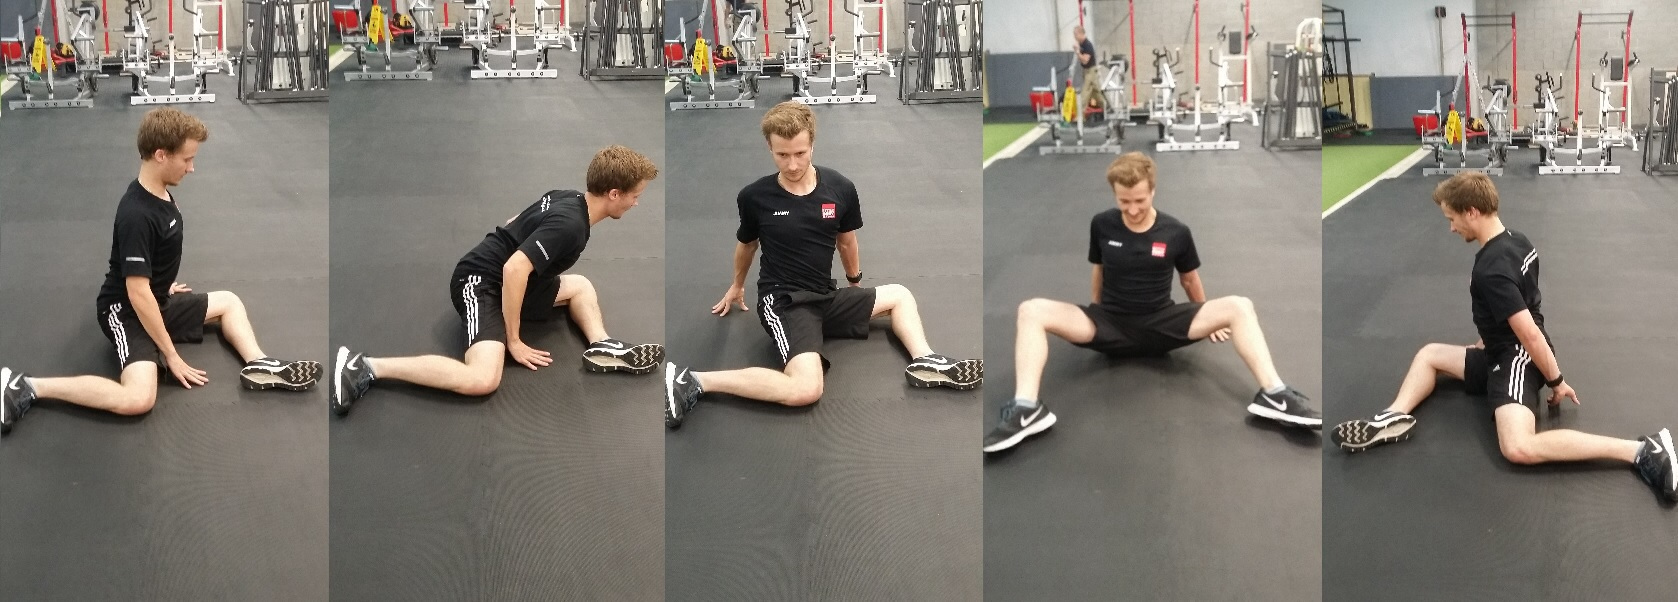
\includegraphics[width=0.8\linewidth]{img/Hueftmobility-betterbodygroup.jpg}
    \caption{Mobilisation der Hüftinnen-Rotation \cite{betterbodygroup}}
    \label{Mobilisation-der-Hueftinnen-Rotation}
\end{figure}

\subsubsection{Ausführung der Übung}

\begin{description}
    \item[$\bullet$ Startposition:]
        \item[$\cdot$ ] Setzen Sie sich auf den Boden, die Beine vor Ihnen angewinkelt
        \item[$\cdot$] Die Fußsohlen zeigen nach oben, die Knie sind leicht gespreizt
    \item[$\bullet$ Bewegung:]
        \item[$\cdot$] Lehnen Sie sich leicht nach hinten, stützen Sie sich mit den Händen ab (wie auf dem Bild rechts)
        \item[$\cdot$]Kippen Sie ein Knie nach innen, während das andere Bein möglichst stabil bleibt
        \item[$\cdot$] Halten Sie die Position für einige Sekunden, kehren Sie dann in die Ausgangsposition zurück und wechseln Sie die Seite
    \item[$\bullet$ Wiederholungen:]Führen Sie die Übung langsam und kontrolliert aus. Jede Seite etwa 8-12 Wiederholungen, in 2-3 Sätzen
\end{description}

\subsubsection{Ziel der Übung}
Durch gezielte Mobilisation wird die Beweglichkeit der weniger beweglichen Seite verbessert, und somit Rechts-Links-Defizite ausgeglichen.
Die Übung fördert außerdem die Hüftinnenrotation, die oft eingeschränkt ist und zu Asymmetrien im Gangbild und bei sportlichen Aktivitäten führen kann.
Schlussendlich beugt die Übung durch das fördern einer besseren Symmetrie der Hüftbewegungen langfristig Hüftproblemen vor.

% \begin{description}
%         \item[$\bullet$ Ausgleich von Rechts-Links-Defiziten:]  Durch gezielte Mobilisation wird die Beweglichkeit der weniger beweglichen Seite verbessert.
%         \item[$\bullet$ Verbesserung der Hüftinnenrotation:]  Diese Bewegung ist oft eingeschränkt, was zu Asymmetrien im Gangbild und bei sportlichen Aktivitäten führen kann.
%         \item[$\bullet$ Prävention von Hüftproblemen:]  Eine bessere Symmetrie der Hüftbewegungen beugt langfristig Überlastungen vor.
% \end{description}

\subsubsection{Was passiert im Körper?}
Diese Übung dient dazu, die Gelenkkapsel der Hüfte in der Innenrotation zu dehnen und zu mobilisieren.
Verkürzte oder verspannte Strukturen, wie das Ligamentum iliofemorale oder die Innenrotatoren, werden dabei durch die kontrollierte Bewegung gedehnt.
Gleichzeitig wird die neuromuskuläre Kontrolle verbessert, indem das Zusammenspiel zwischen stabilisierenden und bewegenden Muskeln trainiert wird.
Zudem trägt die Übung zur Reduzierung von Rechts-Links-Defiziten bei, wodurch die Statik der unteren Extremitäten positiv beeinflusst wird.
Darüber hinaus fördert die Bewegung die Durchblutung der umliegenden Strukturen, was Regeneration und Beweglichkeit unterstützt.

% \begin{description}
%     \item[$\bullet$Mobilisation der Hüftgelenkskapsel]
%         \item[$\cdot$]Die Übung dehnt und mobilisiert die Gelenkkapsel der Hüfte in der Innenrotation
%         \item[$\cdot$] Verkürzte oder verspannte Strukturen, wie das Ligamentum iliofemorale oder die Innenrotatoren, werden durch die kontrollierte Bewegung gedehnt.
%     \item[$\bullet$ Verbesserung der neuromuskulären Kontrolle:] Durch die kontrollierte Bewegung wird das Zusammenspiel zwischen Muskeln, die die Hüfte stabilisieren, und den Bewegungsmuskeln trainiert.
%     \item[$\bullet$ Symmetrie im Bewegungsapparat:] Rechts-Links-Defizite werden gezielt reduziert, was die Statik der gesamten unteren Extremitäten positiv beeinflusst.
%     \item[$\bullet$ Förderung der Durchblutung:] Durch die Bewegung wird die Durchblutung der umliegenden Strukturen verbessert, was die Regeneration und Beweglichkeit fördert.
% \end{description}

\subsection{Heel Down}

Diese Übung wird in der Regel eingesetzt, um die Beinachse, Kraftkontrolle und Stabilität der unteren Extremitäten zu verbessern. Sie fokussiert insbesondere auf die Exzentrik der Muskulatur (kontrolliertes Absenken) und eignet sich ideal zur Behandlung von Dysbalancen zwischen den Beinen oder zur Rehabilitation.

\begin{figure}[!]
    \centering
    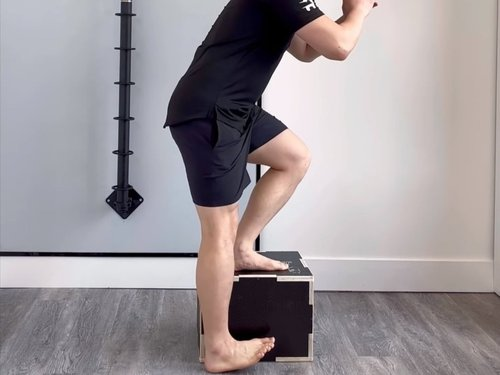
\includegraphics[width=0.5\linewidth]{img/Heel-down-Uebung.jpg}
    \caption{Heel down Ausgleichsübung \cite{rehabhero}}
    \label{Heel-down-Ausgleichsübung}
\end{figure}

\subsubsection{Ausführung der Übung}

\begin{description}
    \item[$\bullet$ Startposition:]
        \item[$\cdot$ ] Stellen Sie sich mit einem Fuß auf eine Erhöhung. Der andere Fuß hängt frei in der Luft.
        \item[$\cdot$ ]Der Körper ist aufrecht, Schultern entspannt und die Arme können seitlich hängen oder leicht zur Balance beitragen.
     \item[$\bullet$ Bewegung:]
        \item[$\cdot$ ] Beugen Sie das Standbein kontrolliert, sodass der freie Fuß nach unten Richtung Boden sinkt.
        \item[$\cdot$ ]Halten Sie dabei die Hüfte und den Oberkörper gerade und stabil.
        \item[$\cdot$ ] Achten Sie darauf, dass die Bewegung langsam und kontrolliert erfolgt.
        \item[$\cdot$ ] Sobald der freie Fuß knapp über dem Boden schwebt, drücken Sie sich durch das Standbein wieder in die Ausgangsposition.
    \item[$\bullet$ Wiederholungen:]Führen Sie pro Seite 10-15 Wiederholungen durch, in 2-3 Sätzen.

\end{description}

\subsubsection{Ziel der Übung}

Die kontrollierte Abwärtsbewegung der Übung fördert die exzentrische Belastung der Muskulatur, insbesondere des Quadriceps, Gluteus und der Waden.
Durch die isolierte Belastung des Standbeins wird dessen Stabilität, besonders in Knie und Hüfte, gestärkt.
Diese Übung trägt ebenfalls zur Reduktion von Asymmetrien bei, indem sie Rechts-Links-Defizite in Kraft und Kontrolle ausgleicht.
Zusätzlich wird die Balance und Propriozeption verbessert, da das Standbein stabilisiert wird, wodurch die Wahrnehmung der Körperhaltung gefördert wird.

% \begin{description}
%     \item[$\bullet$ Verbesserung der exzentrischen Kraft:] Die kontrollierte Abwärtsbewegung trainiert die Muskulatur, insbesondere Quadriceps, Gluteus und Waden, auf exzentrische Belastungen.
%     \item[$\bullet$ Stärkung der Beinachse:] Durch die isolierte Belastung wird die Stabilität des Standbeins gefördert, besonders in Knie und Hüfte.
%     \item[$\bullet$ Reduktion von Asymmetrien:]  Die Übung kann helfen, Rechts-Links-Defizite in Kraft und Kontrolle auszugleichen.
%     \item[$\bullet$ Förderung der Balance und Propriozeption: ] Da das Standbein stabilisiert, wird die Balance und die Wahrnehmung der Körperhaltung verbessert.
% \end{description}

\subsubsection{Was passiert im Körper?}
Die exzentrische Belastung aktiviert intensiv den Quadriceps, der während des Absenkens die Bewegung kontrolliert, während unterstützende Muskeln wie der Gluteus maximus und die Wadenmuskulatur bei der Stabilisierung und Kraftentwicklung helfen.
Die Übung stärkt zudem die muskulären und ligamentären Strukturen im Knie und in der Hüfte, verbessert das Tracking der Patella (Kniescheibe) und reduziert das Risiko von Fehlbelastungen.
Durch die gezielte Kontrolle des Absenkens wird die Koordination und Präzision der Bewegung gefördert, was sowohl im Alltag als auch bei sportlichen Aktivitäten von Vorteil ist.
% \begin{description}
    % \item[$\bullet$ Muskuläre Kontrolle:]

    % \item[$\cdot$] Die exzentrische Belastung aktiviert den Quadriceps intensiv, der während des Absenkens die Bewegung kontrolliert.
    % \item[$\cdot$] Unterstützende Muskeln wie Gluteus maximus und die Wadenmuskulatur helfen bei der Stabilisierung und Kraftentwicklung.

    % \item[$\bullet$ Knie- und Hüftstabilität:]
    %     \item[$\cdot$]Die Übung stärkt die muskulären und ligamentären Strukturen im Knie und in der Hüfte.
    %     \item[$\cdot$]Sie verbessert das Tracking der Patella (Kniescheibe) und reduziert das Risiko von Fehlbelastungen.
    % \item[$\bullet$ Verbesserung der Bewegungsqualität:] Die gezielte Kontrolle des Absenkens fördert die Koordination und die Präzision der Bewegung, was besonders im Alltag und bei sportlichen Aktivitäten hilfreich ist.

% \end{description}

\subsection{Mobilisation Sprunggelenk}

Diese Übung dient der Mobilisation des oberen Sprunggelenks (Dorsalflexion) und der Verbesserung der Beweglichkeit und Stabilität im Fuß- und Knöchelbereich. Sie ist besonders hilfreich, um Bewegungseinschränkungen in der Dorsalflexion zu beheben, die oft Ursache für Knie- oder Hüftprobleme sind.

\begin{figure}
    \centering
    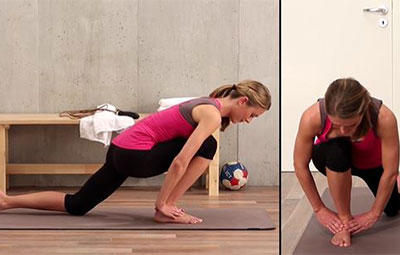
\includegraphics[width=0.5\linewidth]{img/Sprunggelenk-Mobilisation.JPG}
    \caption{Mobilisation Sprunggelenk \cite{valife}}
    \label{Mobilisation-Sprunggelenk}
\end{figure}


\subsubsection{Ausführung der Übung:}

\begin{description}
    \item[$\bullet$ Startposition:]
        \item[$\cdot$]Gehen Sie in den Kniestand
        \item[$\cdot$]Ein Bei ist aufgestellt, der Fuß steht fest auf dem Boden, während das andere Knie am Boden ruht.
        \item[$\cdot$]Die Hände umfassen den Fuß des aufgestellten Beins, um ihn zu stabilisieren.
    \item[$\bullet$ Bewegung: ]
        \item[$\cdot$]Beugen Sie das vordere Knie langsam nach vorne, sodass Sie das Sprunggelenk in die Dorsalflexion bringen(wie auf dem rechten Bild).
        \item[$\cdot$] Achten Sie darauf, dass die Ferse des vorderen Fußes fest am Boden bleibt.
        \item[$\cdot$]Halten Sie die Position für einige Sekunden und kehren Sie langsam in die Ausgangsposition zurück.
    \item[$\bullet$ Wiederholungen: ] Führen Sie 8-12 Wiederholungen pro Bein durch, in 2-3 Sätzen.

\end{description}

\subsubsection{Ziel der Übung}
Die Verbesserung der Sprunggelenk-Mobilität, insbesondere der Dorsalflexion, spielt eine entscheidende Rolle für Bewegungen wie Gehen, Laufen und Kniebeugen, und soll durch diese Übung unterstützt werden.
Zudem fördert die Übung die Stabilisierung des Fußes, indem sie die Kontrolle und Belastungsfähigkeit im Sprunggelenk stärkt.
Darüber hinaus trägt sie zur Prävention und Rehabilitation bei, indem sie Kompensationsbewegungen in Knie und Hüfte durch eingeschränkte Sprunggelenksmobilität vermeidet.

% \begin{description}
%     \item[$\bullet$ Verbesserung der Sprunggelenk-Mobilistät:]  Insbesondere der Dorsalflexion, die für viele Bewegungen wie Gehen, Laufen und Kniebeugen entscheidend ist.
%     \item[$\bullet$ Stabilisierung des Fußes:]  Förderung der Kontrolle und Belastungsfähigkeit im Sprunggelenk.
%     \item[$\bullet$ Prävention und Rehabilitation:]  Vermeidung von Kompensationsbewegungen in Knie und Hüfte durch eingeschränkte Sprunggelenksmobilität.
% \end{description}

\subsubsection{Was passiert im Körper?}
Die Mobilisation des oberen Sprunggelenks trainiert die Gelenkkapsel und dehnt die Wadenmuskulatur, während gleichzeitig das Ligamentum talofibulare anterius (vorderes Band) mobilisiert wird, was die Gelenkmechanik optimiert.
Die Übung verbessert die Dorsalflexion, indem sie Blockaden, die durch Verkürzungen der Wadenmuskulatur oder steife Gelenkstrukturen entstehen können, löst.
Eine bessere Mobilität im Sprunggelenk führt zu einer korrekten Belastung der Knie und Hüfte, wodurch Fehlstellungen und Überbelastungen vermieden werden.

% \begin{description}
%     \item[$\bullet$ Mobilisation des oberen Sprunggelenks:]
%         \item[$\cdot$]Die Bewegung trainiert die Gelenkkapsel und dehnt die Wadenmuskulatur
%         \item[$\cdot$]Gleichzeitig wird das Ligamentum talofibulare anterius (vorderes Bad) mobilisiert, wodurch die Gelenkmechanik optimiert wird.
%     \item[$\bullet$ Verbesserung der Dorsalflexion:] Einschränkungen können durch Verkürzungen der Wadenmuskulatur oder steife Gelenkstrukturen entstehen. Die Übung hilft, diese Blockaden zu lösen.
%     \item[$\bullet$ Förderung der Gelenkmechanik:] Eine bessere Mobilität im Sprunggelenk führt zu einer korrekten Belastung der Knie und Hüfte, wodurch Fehlstellungen und Überbelastungen vermieden werden.
%     \item[$\bullet$]
%     \item[$\bullet$]
% \end{description}







